\documentclass{article}




\usepackage{fullpage}
%\usepackage{nopageno}
\usepackage{amsmath}
\usepackage{amsfonts}
\usepackage{graphicx}
\usepackage{framed}
\usepackage{algorithmic}
\usepackage{xcolor}

\definecolor{dark_red}{rgb}{0.5,0.0,0.0}
\definecolor{dark_green}{rgb}{0.0,0.5,0.0}
\definecolor{dark_blue}{rgb}{0.0,0.0,0.5}
\definecolor{blue}{rgb}{0.0,0.0,1.0}

\newcommand{\dr}[1]{\textcolor{dark_red}{#1}}
\newcommand{\dg}[1]{\textcolor{dark_green}{#1}}
\newcommand{\db}[1]{\textcolor{dark_blue}{#1}}
\newcommand{\blue}[1]{\textcolor{blue}{#1}}


\usepackage{fancyhdr}
%\setlength{\footheight}{15.2pt}
\pagestyle{fancy}
\fancyhead[C]{Wentworth Institute of Technology, MATH2025}
\fancyfoot[C]{Author: Shawn Eastwood}
\renewcommand{\headsep}{25pt}
\renewcommand{\headrulewidth}{1pt}
\renewcommand{\footrulewidth}{1pt}


\begin{document}

\section*{Local minimums and local maximums}

Consider an arbitrary \(n\) parameter function, \(f(x_1, x_2, ..., x_n)\). 

A point \((a_1, a_2, ..., a_n)\) is a {\bf local minimum} of \(f\) if and only if \(f(a_1, a_2, ..., a_n)\) is less than or equal to the values of \(f(x_1, x_2, ..., x_n)\) for all ``nearby" points \((x_1, x_2, ..., x_n)\). If \((x_1, x_2, ..., x_n)\) is ``close" to \((a_1, a_2, ..., a_n)\), then \(f(a_1, a_2, ..., a_n) \leq f(x_1, x_2, ..., x_n)\). 

A point \((a_1, a_2, ..., a_n)\) is a {\bf local maximum} of \(f\) if and only if \(f(a_1, a_2, ..., a_n)\) is greater than or equal to the values of \(f(x_1, x_2, ..., x_n)\) for all ``nearby" points \((x_1, x_2, ..., x_n)\). If \((x_1, x_2, ..., x_n)\) is ``close" to \((a_1, a_2, ..., a_n)\), then \(f(a_1, a_2, ..., a_n) \geq f(x_1, x_2, ..., x_n)\). 




\subsection*{Critical points}

Consider a single variable function \(f(x)\). The ``critical points" of \(f(x)\) are that value of \(x\) that are ``points of interest" that might contain a local minimum or a local maximum. More exactly, the critical points are the values of \(x_0\) where either \(\left.\frac{df}{dx}\right|_{x_0}\) does not exist or \(\left.\frac{df}{dx}\right|_{x_0} = 0\). 

If \(\left.\frac{df}{dx}\right|_{x_0}\) exists, then why must \(\left.\frac{df}{dx}\right|_{x_0} = 0\) at a local minimum or local maximum? If \(\left.\frac{df}{dx}\right|_{x_0} \neq 0\), then for values of \(x\) that are ``close" to \(x_0\), \(f(x) < f(x_0)\) on one side of \(x_0\), and \(f(x) > f(x_0)\) on the other side of \(x_0\) which prevents \(x_0\) from being a local minimum or a local maximum. 

It is at the critical points where local minimums and maximums are located, but not every critical point is a local minimum or maximum.

\begin{center}
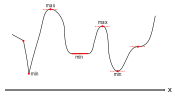
\includegraphics[width = \textwidth]{1_variable_function_critical_points}
\end{center}

Consider the critical points where \(\frac{df}{dx} = 0\). To identify a critical point as a minimum, maximum, or neither, the second derivative at the critical point is examined. 

Let \(x_0\) be an arbitrary value. Let \(c = f(x_0)\), \(b = \left.\frac{df}{dx}\right|_{x_0}\), and \(a = \left.\frac{d^2 f}{dx^2}\right|_{x_0}\). A ``second order" approximation of \(f(x)\) for values of \(x\) that are close to \(x_0\) is:  
\[f(x) \approx c + b(x - x_0) + \frac{1}{2}a(x - x_0)^2\]

When \(\left.\frac{df}{dx}\right|_{x_0} = 0\) at a critical point \(x_0\), the second order approximation becomes:
\[f(x) \approx c + \frac{1}{2}a(x - x_0)^2\]

\begin{tabular}{cc}
\parbox{0.35\textwidth}{  
When \(a > 0\), the second order approximation predicts a minimum at \(x_0\). When \(a < 0\), the second order approximation predicts a maximum at \(x_0\). When \(a = 0\), the second order approximation cannot identify whether \(x_0\) is a minimum, maximum, or neither.
} & \parbox{0.65\textwidth}{
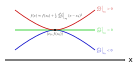
\includegraphics[width = 0.65\textwidth]{1_variable_second_derivative_test}
}
\end{tabular}

When \(\left.\frac{d^2 f}{dx^2}\right|_{x_0} = 0\) and the second derivative test returns no information, there may still exist a local minimum or local maximum at \(x_0\). For example, with respect to the function \(f(x) = x^4\), a local minimum exists at \(x_0 = 0\) even though \(\left.\frac{d^2f}{dx^2}\right|_0 = (12x^2)\Big|_{x = 0} = 0\).

\vspace{5mm}

Now this concept will be generalized to 2 variable functions. Critical points are ``points of interest" where local minimums or local maximums might be found. Let \(f(x, y)\) be an arbitrary function, and let \((x_0, y_0)\) be an arbitrary point. If any of the partial derivatives \(\left.\frac{\partial f}{\partial x}\right|_{(x_0, y_0)}\) and \(\left.\frac{\partial f}{\partial y}\right|_{(x_0, y_0)}\) fails to exist, then \((x_0, y_0)\) is a point of interest and is hence a ``critical point". Now assume that both partial derivatives exist. For \((x_0, y_0)\) to be a local minimum or maximum, both partial derivatives \(\left.\frac{\partial f}{\partial x}\right|_{(x_0, y_0)}\) and \(\left.\frac{\partial f}{\partial y}\right|_{(x_0, y_0)}\) must be \(0\). The reason for this is as follows: If for example, \(\left.\frac{\partial f}{\partial x}\right|_{(x_0, y_0)} > 0\), then increasing \(x\) from \(x_0\) by a small amount will increase \(f(x, y)\), and decreasing \(x\) from \(x_0\) by a small amount will decrease \(f(x, y)\). This prevents \((x_0, y_0)\) from being a local minimum or maximum. {\bf The point \((x_0, y_0)\) is a critical point if and only if one of the partial derivatives fails to exist, or \(\left.\frac{\partial f}{\partial x}\right|_{(x_0, y_0)} = 0\) and \(\left.\frac{\partial f}{\partial y}\right|_{(x_0, y_0)} = 0\).}

Once critical points have been found, now they need to be identified as local minimums, local maximums, or neither. Only critical points \((x_0, y_0)\) where both partial derivatives \(\left.\frac{\partial f}{\partial x}\right|_{(x_0, y_0)}\) and \(\left.\frac{\partial f}{\partial y}\right|_{(x_0, y_0)}\) exist and are both equal to \(0\) will be classified by examination of the second partial derivatives, ``the second derivative test". 

Assume that the first and second partial derivatives all exist. Let 

\begin{tabular}{ccc}
\(c = f(x_0, y_0)\) & \(b_x = \left.\frac{\partial f}{\partial x}\right|_{(x_0, y_0)}\) & \(b_y = \left.\frac{\partial f}{\partial y}\right|_{(x_0, y_0)}\) \\
\(a_{xx} = \left.\frac{\partial^2 f}{\partial x^2}\right|_{(x_0, y_0)}\) & \(a_{xy} = \left.\frac{\partial^2 f}{\partial x \partial y}\right|_{(x_0, y_0)}\) & \(a_{yy} = \left.\frac{\partial^2 f}{\partial y^2}\right|_{(x_0, y_0)}\)  
\end{tabular}

The second order approximation of \(f(x,y)\) for \((x, y)\) ``close" to \((x_0, y_0)\) is:
\[f(x, y) \approx c + b_x(x - x_0) + b_y(y - y_0) + \frac{1}{2}a_{xx}(x - x_0)^2 + a_{xy}(x - x_0)(y - y_0) + \frac{1}{2}a_{yy}(y - y_0)^2\]

At a critical point where \(b_x = 0\) and \(b_y = 0\), the second order approximation becomes: 
\[f(x, y) \approx c + \frac{1}{2}a_{xx}(x - x_0)^2 + a_{xy}(x - x_0)(y - y_0) + \frac{1}{2}a_{yy}(y - y_0)^2\]

{\bf The following framed discussion is for the purpose of completion and can be safely skipped.}

\begin{framed}
Let \(\epsilon\) be a small positive value (\(\epsilon > 0\)), and let \(\theta\) denote an arbitrary angle. The point 
\[(x, y) = (x_0 + \epsilon \cos\theta, y_0 + \epsilon \sin\theta)\] 
is an arbitrary point that is exactly a distance of \(\epsilon\) from \((x_0, y_0)\). The value of \(f(x, y)\) given by the second order approximation is: 
\begin{align*}
f(x, y) = & f(x_0 + \epsilon \cos\theta, y_0 + \epsilon \sin\theta) \\
\approx & c + \frac{1}{2}a_{xx}(\epsilon \cos\theta)^2 + a_{xy}(\epsilon \cos\theta)(\epsilon \sin\theta) + \frac{1}{2}a_{yy}(\epsilon \sin\theta)^2 \\
= & c + \epsilon^2(\frac{1}{2}a_{xx}\cos^2\theta + a_{xy}\cos\theta\sin\theta + \frac{1}{2}a_{yy}\sin^2\theta) \\
= & c + \epsilon^2(\frac{1}{2}(a_{xx} - a_{yy})\cos^2\theta + a_{xy}\cos\theta\sin\theta + \frac{1}{2}a_{yy}(\cos^2\theta + \sin^2\theta)) \\
= & c + \epsilon^2(\frac{1}{2}a_{yy} + \frac{1}{2}(a_{xx} - a_{yy})\cos^2\theta + a_{xy}\cos\theta\sin\theta) \\ 
= & c + \epsilon^2(\frac{1}{2}a_{yy} + \frac{1}{2}(a_{xx} - a_{yy})\frac{\cos(2\theta) + 1}{2} + a_{xy}\frac{\sin(2\theta)}{2}) \\ 
= & c + \epsilon^2(\frac{1}{4}(a_{xx} + a_{yy}) + \frac{1}{4}(a_{xx} - a_{yy})\cos(2\theta) + \frac{1}{2}a_{xy}\sin(2\theta)) 
\end{align*}

For simplicity, define the function \(g(\theta) = \dr{\frac{1}{4}(a_{xx} + a_{yy})} + \dg{\frac{1}{4}(a_{xx} - a_{yy})\cos(2\theta) + \frac{1}{2}a_{xy}\sin(2\theta)}\) so \(f(x, y) = c + \epsilon^2 g(\theta)\).

\vspace{2mm}

If \(g(\theta) > 0\) for all \(\theta\), then \(f(x, y) > c = f(x_0, y_0)\) for all \((x, y)\) ``close" to \((x_0, y_0)\) and \((x_0, y_0)\) is therefore a local minimum. 

\vspace{2mm}

If \(g(\theta) < 0\) for all \(\theta\), then \(f(x, y) < c = f(x_0, y_0)\) for all \((x, y)\) ``close" to \((x_0, y_0)\) and \((x_0, y_0)\) is therefore a local maximum. 

\vspace{2mm}

If \(g(\theta)\) attains a mix of positive and negative values, then \(f(x, y)\) is both greater than \(c\) for some \((x, y)\) ``close" to \((x_0, y_0)\), and \(f(x,y)\) is less than \(c\) for other \((x, y)\) ``close" to \((x_0, y_0)\). The critical point \((x_0, y_0)\) is therefore a {\bf saddle point}. 

\vspace{2mm}

If \(g(\theta)\) touches \(0\) but is not a mix of positive and negative values, then no information about the critical point \((x_0, y_0)\) can be concluded. 

\vspace{2mm}

To analyze the values attained by \(g(\theta)\), the size of the sinusoidal components will be compared to the constant component.

\vspace{2mm}

The constant term from \(g(\theta)\) is \(\dr{\frac{1}{4}(a_{xx} + a_{yy})}\). 

\vspace{2mm}

\(\dg{\frac{1}{4}(a_{xx} - a_{yy})\cos(2\theta) + \frac{1}{2}a_{xy}\sin(2\theta)}\) is a sinusoidal function of \(\theta\). The amplitude of this sinusoidal function is:
\begin{align*}
& \sqrt{\left(\frac{1}{4}(a_{xx} - a_{yy})\right)^2 + \left(\frac{1}{2}a_{xy}\right)^2} 
= \frac{1}{4}\sqrt{a_{xx}^2 - 2a_{xx}a_{yy} + a_{yy}^2 + 4a_{xy}^2}
\end{align*}

If the absolute value of the constant term from \(g(\theta)\) is greater than the amplitude, then \(g(\theta)\) is either strictly positive for all \(\theta\), or strictly negative for all \(\theta\). This condition is: 
\begin{align*}
& \left|\frac{1}{4}(a_{xx} + a_{yy})\right| > \frac{1}{4}\sqrt{a_{xx}^2 - 2a_{xx}a_{yy} + a_{yy}^2 + 4a_{xy}^2} \\ 
& \iff |a_{xx} + a_{yy}| > \sqrt{a_{xx}^2 - 2a_{xx}a_{yy} + a_{yy}^2 + 4a_{xy}^2} \\ 
& \iff a_{xx}^2 + 2a_{xx}a_{yy} + a_{yy}^2 > a_{xx}^2 - 2a_{xx}a_{yy} + a_{yy}^2 + 4a_{xy}^2 \\ 
& \iff a_{xx}a_{yy} > a_{xy}^2
\end{align*}
If the absolute value of the constant term from \(g(\theta)\) is less than the amplitude, then \(g(\theta)\) is a mix of positive and negative values. This condition is:
\[a_{xx}a_{yy} < a_{xy}^2\] 
If the absolute value of the constant term from \(g(\theta)\) is equal to the amplitude, then \(g(\theta)\) touches \(0\) but is not a mix of positive and negative values. This condition is:
\[a_{xx}a_{yy} = a_{xy}^2\] 
The quantity \(\Delta = a_{xx}a_{yy} - a_{xy}^2\) can be used to discriminate between the possible scenarios.
\end{framed}

Compute the ``discriminant" 
\[\Delta = a_{xx} a_{yy} - a_{xy}^2\]
\begin{itemize}
\item If \(\Delta > 0\), then the critical point \((x_0, y_0)\) is a local minimum or a local maximum. Note that \(a_{xx}\) and \(a_{yy}\) must have the same sign for \(\Delta > 0\) to be possible. The common sign will determine whether the critical point is a local minimum or local maximum.  
\begin{itemize}
\item[*] If \(a_{xx} > 0\) then \((x_0, y_0)\) is a local minimum. 
\item[*] If \(a_{xx} < 0\) then \((x_0, y_0)\) is a local maximum. 
\end{itemize}
\item If \(\Delta < 0\), then the critical point \((x_0, y_0)\) is a {\bf saddle point}. A saddle point is a critical point where \(\left.\frac{\partial f}{\partial x}\right|_{(x_0, y_0)}\) and \(\left.\frac{\partial f}{\partial y}\right|_{(x_0, y_0)}\) both exist and are both equal to \(0\), but is surrounded by points that are both greater than or less than \(f(x_0, y_0)\).
\item If \(\Delta = 0\), then no information about the critical point is acquired. 
\end{itemize}

\vspace{5mm}

\textbf{Examples:}
\begin{itemize}
%%%%%%%%%%%%%%%%%%%%
\item** Find and classify the critical points of the function:
\[f(x,y) = -x^3 + 4xy - 2y^2 + 1\]
The gradient is:
\[\nabla f = \begin{bmatrix} \partial f/\partial x \\ \partial f/\partial y \end{bmatrix} = \begin{bmatrix} -3x^2 + 4y \\ 4x - 4y \end{bmatrix}\]
The critical points are the values of \((x_0, y_0)\) where both partial derivatives are \(0\):
\begin{align*}
& (\nabla f)\Big|_{(x_0, y_0)} = 0 
\iff \left\{\begin{array}{c} (\partial f/\partial x)|_{(x_0, y_0)} = 0 \\ (\partial f/\partial y)|_{(x_0, y_0)} = 0 \end{array}\right. 
\iff \left\{\begin{array}{c} -3x_0^2 + 4y_0 = 0 \\ 4x_0 - 4y_0 = 0 \end{array}\right. 
\end{align*}
Solving the second equation for \(y_0\) gives: 
\[4x_0 - 4y_0 = 0 \iff y_0 = x_0\]
Replacing \(y_0\) in the first equation gives:
\begin{align*} 
& -3x_0^2 + 4x_0 = 0 
\iff x_0(-3x_0 + 4) = 0 
\iff (x_0 = 0) \;\text{or}\; (-3x_0 + 4 = 0) 
\iff (x_0 = 0) \;\text{or}\; (x_0 = 4/3) 
\end{align*}  
There are two values of \(x_0\): i.e. \(x_0 = 0, 4/3\)

The corresponding values of \(y_0\) are: \(y_0 = 0, 4/3\) 

There are two critical points:
\[(x_0, y_0) = (0, 0) \quad\quad\text{and}\quad\quad (x_0, y_0) = (4/3, 4/3)\]

The second order partial derivatives are:
\[\frac{\partial^2 f}{\partial x^2} = -6x \quad\quad\text{and}\quad\quad \frac{\partial^2 f}{\partial x \partial y} = 4 \quad\quad\text{and}\quad\quad \frac{\partial^2 f}{\partial y^2} = -4\]

At the critical point \((0, 0)\), the discriminant is:
\[\Delta = \left(\left.\frac{\partial^2 f}{\partial x^2}\right|_{(0,0)}\right)\left(\left.\frac{\partial^2 f}{\partial y^2}\right|_{(0,0)}\right) - \left(\left.\frac{\partial^2 f}{\partial x \partial y}\right|_{(0,0)}\right)^2 = (0)(-4) - (4)^2 = -16\]
\(\Delta < 0\) so \((0, 0)\) is a ``saddle point".

At the critical point \((4/3, 4/3)\), the discriminant is:
\[\Delta = \left(\left.\frac{\partial^2 f}{\partial x^2}\right|_{(4/3, 4/3)}\right)\left(\left.\frac{\partial^2 f}{\partial y^2}\right|_{(4/3, 4/3)}\right) - \left(\left.\frac{\partial^2 f}{\partial x \partial y}\right|_{(4/3, 4/3)}\right)^2 = (-8)(-4) - (4)^2 = 16\]
\(\Delta > 0\) and \(\left.\frac{\partial^2 f}{\partial x^2}\right|_{(4/3, 4/3)} < 0\) so \((4/3, 4/3)\) is a local maximum.

\begin{center}
\includegraphics[width = 0.5\textwidth]{critical_points_1.png}
\end{center}

%%%%%%%%%%%%%%%%%%%%
\item Find and classify the critical points of the function:
\[f(x,y) = -\frac{3}{4}y^3 - x^2 + 3xy + \frac{9}{4}y^2 - 5x + \frac{3}{4}y - 10\]
The gradient is:
\[\nabla f = \begin{bmatrix} \partial f/\partial x \\ \partial f/\partial y \end{bmatrix} = \begin{bmatrix} -2x + 3y - 5 \\ -\frac{9}{4}y^2 + 3x + \frac{9}{2}y + \frac{3}{4} \end{bmatrix}\]
The critical points are the values of \((x_0, y_0)\) where both partial derivatives are \(0\):
\begin{align*}
& (\nabla f)\Big|_{(x_0, y_0)} = 0 
\iff \left\{\begin{array}{c} (\partial f/\partial x)|_{(x_0, y_0)} = 0 \\ (\partial f/\partial y)|_{(x_0, y_0)} = 0 \end{array}\right. 
\iff \left\{\begin{array}{c} -2x_0 + 3y_0 - 5 = 0 \\ -\frac{9}{4}y_0^2 + 3x_0 + \frac{9}{2}y_0 + \frac{3}{4} = 0 \end{array}\right. 
\end{align*}
Solving the first equation for \(y_0\) gives: 
\[-2x_0 + 3y_0 - 5 = 0 \iff 3y_0 = 2x_0 + 5 \iff y_0 = \frac{2}{3}x_0 + \frac{5}{3}\]
Replacing \(y_0\) in the second equation gives:
\begin{align*} 
& -\frac{9}{4}(\frac{2}{3}x_0 + \frac{5}{3})^2 + 3x_0 + \frac{9}{2}(\frac{2}{3}x_0 + \frac{5}{3}) + \frac{3}{4} = 0 \\ 
& \iff -\frac{9}{4}(\frac{4}{9}x_0^2 + \frac{20}{9}x_0 + \frac{25}{9}) + 3x_0 + (3x_0 + \frac{15}{2}) + \frac{3}{4} = 0 \\  
& \iff (-x_0^2 - 5x_0 - \frac{25}{4}) + (6x_0 + \frac{33}{4}) = 0 \\
& \iff -x_0^2 + x_0 + 2 = 0 
\iff x_0 = \frac{-1 \pm \sqrt{1 + 8}}{-2} = \frac{-1 \pm 3}{-2} = -1, 2
\end{align*}  
There are two values of \(x_0\): i.e. \(x_0 = -1, 2\)

The corresponding values of \(y_0\) are: \(y_0 = 1, 3\) 

There are two critical points:
\[(x_0, y_0) = (-1, 1) \quad\quad\text{and}\quad\quad (x_0, y_0) = (2, 3)\]

The second order partial derivatives are:
\[\frac{\partial^2 f}{\partial x^2} = -2 \quad\quad\text{and}\quad\quad \frac{\partial^2 f}{\partial x \partial y} = 3 \quad\quad\text{and}\quad\quad \frac{\partial^2 f}{\partial y^2} = -\frac{9}{2}y + \frac{9}{2}\]

At the critical point \((-1,1)\), the discriminant is:
\[\Delta = \left(\left.\frac{\partial^2 f}{\partial x^2}\right|_{(-1,1)}\right)\left(\left.\frac{\partial^2 f}{\partial y^2}\right|_{(-1,1)}\right) - \left(\left.\frac{\partial^2 f}{\partial x \partial y}\right|_{(-1,1)}\right)^2 = (-2)(0) - (3)^2 = -9\]
\(\Delta < 0\) so \((-1, 1)\) is a ``saddle point".

At the critical point \((2,3)\), the discriminant is:
\[\Delta = \left(\left.\frac{\partial^2 f}{\partial x^2}\right|_{(2,3)}\right)\left(\left.\frac{\partial^2 f}{\partial y^2}\right|_{(2,3)}\right) - \left(\left.\frac{\partial^2 f}{\partial x \partial y}\right|_{(2,3)}\right)^2 = (-2)(-9) - (3)^2 = 9\]
\(\Delta > 0\) and \(\left.\frac{\partial^2 f}{\partial x^2}\right|_{(2,3)} < 0\) so \((2, 3)\) is a local maximum.

\begin{center}
\includegraphics[width = 0.5\textwidth]{critical_points_2.png}
\end{center}

%%%%%%%%%%%%%%%%%%%%
\item Find and classify the critical points of the function:
\[f(x,y) = -\frac{2}{3}y^3 + \frac{1}{2}x^2 + 2xy + 14y^2 - 13x - 96y + 25\]
The gradient is:
\[\nabla f = \begin{bmatrix} \partial f/\partial x \\ \partial f/\partial y \end{bmatrix} = \begin{bmatrix} x + 2y - 13 \\ -2y^2 + 2x + 28y - 96 \end{bmatrix}\]
The critical points are the values of \((x_0, y_0)\) where both partial derivatives are \(0\):
\begin{align*}
& (\nabla f)\Big|_{(x_0, y_0)} = 0 
\iff \left\{\begin{array}{c} (\partial f/\partial x)|_{(x_0, y_0)} = 0 \\ (\partial f/\partial y)|_{(x_0, y_0)} = 0 \end{array}\right. 
\iff \left\{\begin{array}{c} x_0 + 2y_0 - 13 = 0 \\ -2y_0^2 + 2x_0 + 28y_0 - 96 = 0 \end{array}\right. 
\end{align*}
Solving the first equation for \(y_0\) gives: 
\[x_0 + 2y_0 - 13 = 0 \iff 2y_0 = -x_0 + 13 \iff y_0 = -\frac{1}{2}x_0 + \frac{13}{2}\]
Replacing \(y_0\) in the second equation gives:
\begin{align*} 
& -2(-\frac{1}{2}x_0 + \frac{13}{2})^2 + 2x_0 + 28(-\frac{1}{2}x_0 + \frac{13}{2}) - 96 = 0 \\  
& \iff -2(\frac{1}{4}x_0^2 - \frac{13}{2}x_0 + \frac{169}{4}) + 2x_0 + (-14x_0 + 182) - 96 = 0 \\
& \iff (-\frac{1}{2}x_0^2 + 13x_0 - \frac{169}{2}) - 12x_0 + 86 = 0 \\ 
& \iff -\frac{1}{2}x_0^2 + x_0 + \frac{3}{2}  = 0  
\iff x_0 = \frac{-1 \pm \sqrt{1 + 3}}{-1} = 1 \mp 2 = -1, 3
\end{align*}  
There are two values of \(x_0\): i.e. \(x_0 = -1, 3\)

The corresponding values of \(y_0\) are: \(y_0 = 7, 5\) 

There are two critical points:
\[(x_0, y_0) = (-1, 7) \quad\quad\text{and}\quad\quad (x_0, y_0) = (3, 5)\]

The second order partial derivatives are:
\[\frac{\partial^2 f}{\partial x^2} = 1 \quad\quad\text{and}\quad\quad \frac{\partial^2 f}{\partial x \partial y} = 2 \quad\quad\text{and}\quad\quad \frac{\partial^2 f}{\partial y^2} = -4y + 28\] 

At the critical point \((-1, 7)\), the discriminant is:
\[\Delta = \left(\left.\frac{\partial^2 f}{\partial x^2}\right|_{(-1, 7)}\right)\left(\left.\frac{\partial^2 f}{\partial y^2}\right|_{(-1, 7)}\right) - \left(\left.\frac{\partial^2 f}{\partial x \partial y}\right|_{(-1, 7)}\right)^2 = (1)(0) - (2)^2 = -4\]
\(\Delta < 0\) so \((-1, 7)\) is a ``saddle point".

At the critical point \((3,5)\), the discriminant is:
\[\Delta = \left(\left.\frac{\partial^2 f}{\partial x^2}\right|_{(3,5)}\right)\left(\left.\frac{\partial^2 f}{\partial y^2}\right|_{(3,5)}\right) - \left(\left.\frac{\partial^2 f}{\partial x \partial y}\right|_{(3,5)}\right)^2 = (1)(8) - (2)^2 = 4\]
\(\Delta > 0\)  and \(\left.\frac{\partial^2 f}{\partial x^2}\right|_{(3,5)} > 0\) so \((3, 5)\) is a local minimum.

\begin{center}
\includegraphics[width = 0.5\textwidth]{critical_points_3.png}
\end{center}

%%%%%%%%%%%%%%%%%%%%
\item** Find and classify the critical points of the function:
\[f(x,y) = 8xy(x + y) + 7\]
The gradient is:
\[\nabla f = \begin{bmatrix} \partial f/\partial x \\ \partial f/\partial y \end{bmatrix} = \begin{bmatrix} 16xy + 8y^2 \\ 8x^2 + 16xy \end{bmatrix}\]
The critical points are the values of \((x_0, y_0)\) where both partial derivatives are \(0\):
\begin{align*}
& (\nabla f)\Big|_{(x_0, y_0)} = 0 
\iff \left\{\begin{array}{c} (\partial f/\partial x)|_{(x_0, y_0)} = 0 \\ (\partial f/\partial y)|_{(x_0, y_0)} = 0 \end{array}\right. 
\iff \left\{\begin{array}{c} 16x_0y_0 + 8y_0^2 = 0 \\ 8x_0^2 + 16x_0y_0 = 0 \end{array}\right. 
\end{align*}
Solving the first equation for \(y_0\) gives: 
\[16x_0y_0 + 8y_0^2 = 0 \iff y_0(2x_0 + y_0) = 0 \iff (y_0 = 0) \;\text{or}\; (y_0 = -2x_0)\]

Replacing \(y_0\) with \(0\) in the second equation gives:
\begin{align*} 
& 8x_0^2 + 16x_0(0) = 0 
\iff x_0^2 = 0 
\iff x_0 = 0
\end{align*}  
One critical point is: \((x_0, y_0) = (0, 0)\). 

Replacing \(y_0\) with \(-2x_0\) in the second equation gives:
\begin{align*} 
& 8x_0^2 + 16x_0(-2x_0) = 0 
\iff -24x_0^2 = 0 
\iff x_0^2 = 0
\iff x_0 = 0
\end{align*}  
The same critical point is generated: \((x_0, y_0) = (0, 0)\).

There is one critical point:
\[(x_0, y_0) = (0, 0)\]

The second order partial derivatives are:
\[\frac{\partial^2 f}{\partial x^2} = 16y \quad\quad\text{and}\quad\quad \frac{\partial^2 f}{\partial x \partial y} = 16x + 16y \quad\quad\text{and}\quad\quad \frac{\partial^2 f}{\partial y^2} = 16x\]

At the critical point \((0, 0)\), the discriminant is:
\[\Delta = \left(\left.\frac{\partial^2 f}{\partial x^2}\right|_{(0,0)}\right)\left(\left.\frac{\partial^2 f}{\partial y^2}\right|_{(0,0)}\right) - \left(\left.\frac{\partial^2 f}{\partial x \partial y}\right|_{(0,0)}\right)^2 = (0)(0) - (0)^2 = 0\]
\(\Delta = 0\) so \((0, 0)\) cannot be classified. The image below however, shows that \((0, 0)\) is in fact a ``saddle point". 

\begin{center}
\includegraphics[width = 0.5\textwidth]{critical_points_4.png}
\end{center}

\end{itemize}
**Examples are from: \\
Strang, G. et. al., ``Calculus Volume 3", \emph{Openstax}, Chapter 4.7 





\section*{Absolute minimums and absolute maximums}

Consider an arbitrary \(n\) parameter function, \(f(x_1, x_2, ..., x_n)\), and a domain \(R \subseteq \mathbb{R}^n\). 

A point \((a_1, a_2, ..., a_n)\) is an {\bf absolute minimum} of \(f\) over the domain \(R\) if and only if \(f(a_1, a_2, ..., a_n)\) is less than or equal to the values of \(f(x_1, x_2, ..., x_n)\) for all points \((x_1, x_2, ..., x_n)\) from set \(R\). If \((x_1, x_2, ..., x_n) \in R\), then \(f(a_1, a_2, ..., a_n) \leq f(x_1, x_2, ..., x_n)\). 

A point \((a_1, a_2, ..., a_n)\) is an {\bf absolute maximum} of \(f\) over the domain \(R\) if and only if \(f(a_1, a_2, ..., a_n)\) is greater than or equal to the values of \(f(x_1, x_2, ..., x_n)\) for all points \((x_1, x_2, ..., x_n)\) from set \(R\). If \((x_1, x_2, ..., x_n) \in R\), then \(f(a_1, a_2, ..., a_n) \geq f(x_1, x_2, ..., x_n)\). 



\subsection*{Lagrange multipliers}

How can the absolute minimum and absolute maximum points be determined? To find the absolute minimum and the absolute maximum, a list \(P_1, P_2, ..., P_m\) of ``candidate points" from the domain \(R\) must be computed. The values of \(f(x_1, x_2, ..., x_n)\) at each of these candidate points, \(f(P_1)\), \(f(P_2)\), ..., \(f(P_m)\) must be computed and the point(s) that give the smallest value of \(f(x_1, x_2, ..., x_n)\) are the absolute minimum points, while the point(s) that give the largest value of \(f(x_1, x_2, ..., x_n)\) are the absolute maximum points.  

The candidate points for the absolute minimum and the absolute maximum consist of the critical points and every possible boundary point. 

For a single variable function \(f(x)\), there are a small number of boundary points. If \(R\) is simply an interval, then there are only 2 boundary points. The image below shows a single variable function with a finite interval domain. All of the candidate points, i.e. the critical points and the boundary points, are highlighted.

\begin{center}
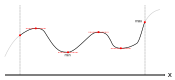
\includegraphics[width = \textwidth]{1_variable_constrained_optimization}
\end{center}

When \(f\) has 2 or more parameters, the boundary of \(R\) consists of an infinite number of points. To narrow down the range of candidate points on the boundary, the absolute minimum and maximum points of \(f\) where the domain has been further restricted to the boundary itself will be computed. In the image below on the left, the critical points on the interior of \(R\) are shown, together with the absolute minimum and absolute maximum points on the boundary of \(R\). In the image below on the right, the computation of the absolute minimum and absolute maximum points of \(f\) on the boundary of \(R\) by amassing a set of candidate points is shown. This section will focus on computing the absolute minimum and absolute maximum points of \(f\) on the boundary of \(R\). 

\begin{center}
\begin{tabular}{cc}
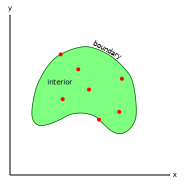
\includegraphics[width = 0.5\textwidth]{2_variable_constrained_optimization} & 
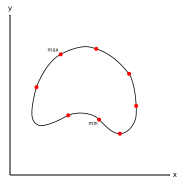
\includegraphics[width = 0.5\textwidth]{2_variable_constrained_optimization_boundary}
\end{tabular}
\end{center}

Consider the \(n\) parameter function \(f(x_1, x_2, ..., x_n)\). The absolute minimum and the absolute maximum value of \(f(x_1, x_2, ..., x_n)\) where \((x_1, x_2, ..., x_n)\) must satisfy \(g(x_1, x_2, ..., x_n) = c\) is sought. The condition \(g(x_1, x_2, ..., x_n) = c\) limits the possible points to the ``surface" defined by the implicit equation \(g(x_1, x_2, ..., x_n) = c\).

Let \(P = (a_1, a_2, ..., a_n)\) denote a ``candidate point". What properties must a candidate point \(P\) satisfy? 

Firstly, \(P = (a_1, a_2, ..., a_n)\) must satisfy the given constraint \(g(P) = g(a_1, a_2, ..., a_n) = c\). 

Next, let \(\mathbf{q}(t) = \begin{bmatrix} q_1(t) \\ q_2(t) \\ \vdots \\ q_n(t) \end{bmatrix}\) denote a vector valued function where \(\mathbf{q}(0) = P = \begin{bmatrix} a_1 \\ a_2 \\ \vdots \\ a_n \end{bmatrix}\) at \(t = 0\), and every point generated by \(\mathbf{q}(t)\) satisfies the constraint: \(g(\mathbf{q}(t)) = c\). Since \(g(\mathbf{q}(t))\) is constant, \(\frac{d}{dt}(g(\mathbf{q}(t))) = 0\). Using the multivariable chain rule, 
\begin{align*} 
\frac{d}{dt}(g(\mathbf{q}(t))) = 0 & \iff \left.\frac{\partial g}{\partial x_1}\right|_{\mathbf{q}(t)}\frac{dq_1}{dt} + \left.\frac{\partial g}{\partial x_2}\right|_{\mathbf{q}(t)}\frac{dq_2}{dt} + ... + \left.\frac{\partial g}{\partial x_n}\right|_{\mathbf{q}(t)}\frac{dq_n}{dt} = 0 \\
& \iff (\nabla g)\Big|_{\mathbf{q}(t)} \bullet \frac{d\mathbf{q}}{dt} = 0
\end{align*}
When \(t = 0\) at point \(P\), the above equation gives \((\nabla g)\Big|_{P} \bullet \left.\frac{d\mathbf{q}}{dt}\right|_{t = 0} = 0\). 

It should also be expected that \(\left.\frac{d}{dt}(f(\mathbf{q}(t)))\right|_{t = 0} = 0\) at \(t = 0\). Why? If \(\left.\frac{d}{dt}(f(\mathbf{q}(t)))\right|_{t = 0} \neq 0\), then for values of \(t\) ``close" to \(0\), \(f(\mathbf{q}(t)) > f(P)\) for values of \(t\) on one side of \(0\), and \(f(\mathbf{q}(t)) < f(P)\) for values of \(t\) on the other side of \(0\). This precludes the possibility of \(P\) being an absolute minimum or maximum of function \(f\). 

From \(\left.\frac{d}{dt}(f(\mathbf{q}(t)))\right|_{t = 0} = 0\) the multivariable chain rule again derives \((\nabla f)\Big|_{P} \bullet \left.\frac{d\mathbf{q}}{dt}\right|_{t = 0} = 0\)

It is now known that at each candidate point, that: 
\[(\nabla g)\Big|_{P} \bullet \left.\frac{d\mathbf{q}}{dt}\right|_{t = 0} = 0 \quad\quad\text{and}\quad\quad (\nabla f)\Big|_{P} \bullet \left.\frac{d\mathbf{q}}{dt}\right|_{t = 0} = 0\]
no matter the choice of \(\left.\frac{d\mathbf{q}}{dt}\right|_{t = 0}\), provided that \(\mathbf{q}(t)\) satisfies the constraint: \(g(\mathbf{q}(t)) = c\). The only way that \((\nabla f)\Big|_{P} \bullet \left.\frac{d\mathbf{q}}{dt}\right|_{t = 0}\) and \((\nabla g)\Big|_{P} \bullet \left.\frac{d\mathbf{q}}{dt}\right|_{t = 0}\) can both always be \(0\) simultaneously if for \((\nabla f)\Big|_{P}\) and \((\nabla g)\Big|_{P}\) to be multiples of each other. The must exist some coefficient \(\lambda\), referred to as a {\bf Lagrange multiplier}, such that:
\[(\nabla f)\Big|_{P} = \lambda (\nabla g)\Big|_{P}\]

Finding all candidate points involves finding all solutions \((a_1, a_2, ..., a_n; \lambda)\) (there are \(n+ 1\) unknowns) of the system of \(n + 1\) equations:
\[\left\{\begin{array}{c}
(\nabla f)\Big|_{(a_1, a_2, ..., a_n)} = \lambda (\nabla g)\Big|_{(a_1, a_2, ..., a_n)} \\ 
g(a_1, a_2, ..., a_n) = c
\end{array}\right.\]
(The first ``equation" is actually \(n\) equations.)

Once all of the candidate points have been gathered, the values of \(f\) are computed at each candidate point, and from the candidate points, the absolute minimum and the absolute maximum are chosen.

\begin{tabular}{cc}
\parbox{0.5\textwidth}{
In the image to the right, the level curves (contour lines) of a 2 parameter function \(f(x,y)\) are shown, along with a constraint curve \(g(x,y) = c\). The image illustrates how at the absolute maximum and minimum, the gradient of \(f(x,y)\), denoted by the dark arrows, is parallel to the gradient of \(g(x,y)\), denoted by the orange arrows. Recall that the gradient vector is always perpendicular to the level curves, and that \(g(x,y) = c\) is a level curve of \(g(x,y)\).
} & \parbox{0.5\textwidth}{
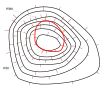
\includegraphics[width = 0.5\textwidth]{level_curves_and_Lagrange_multipliers}
}
\end{tabular}

\vspace{5mm}

\textbf{Examples:}
\begin{itemize}
%%%%%%%%%%%%%%%%%%%%%%%%%%%
\item** Optimize the function:
\[f(x,y) = x + 2y\]
subject to the constraint:
\[18x^2 + 9y^2 = 2\]
Let \(g(x,y) = 18x^2 + 9y^2\).

The gradients of \(f(x, y)\) and \(g(x, y)\) are respectively:

\[\nabla f = \begin{bmatrix}
1 \\ 
2 
\end{bmatrix}
\quad\quad\text{and}\quad\quad
\nabla g = \begin{bmatrix}
36x \\ 
18y 
\end{bmatrix}\]

Candidate points \((x_0, y_0)\) and a Lagrange multiplier \(\lambda\) such that:
\[(\nabla f)\Big|_{(x_0,y_0)} = \lambda (\nabla g)\Big|_{(x_0, y_0)} 
\quad\quad\text{and}\quad\quad 
g(x_0, y_0) = 2\]
need to be solved for. These conditions form a system of 3 equations:
\[\left\{\begin{array}{c}
1 = \lambda (36x_0) \\ 
2 = \lambda (18y_0) \\ 
18x_0^2 + 9y_0^2 = 2
\end{array}\right.\]
which must be solved for the 3 variables \((x_0, y_0; \lambda)\).

The first equation can be solved for \(\lambda = \frac{1}{36x_0}\). What if \(x_0 = 0\)? Two scenarios will now be addressed: \(x_0 = 0\) and \(x_0 \neq 0\).  
\begin{itemize}
\item[*] 
When \(x_0 = 0\), the system reduces to:
\[\left\{\begin{array}{c}
1 = 0 \\ 
2 = \lambda (18y_0) \\ 
9y_0^2 = 2
\end{array}\right.\]
The first equation is a contradiction so \(x_0 \neq 0\). 
\item[*] 
When \(x_0 \neq 0\), the system remains unchanged:
\[\left\{\begin{array}{c}
1 = \lambda (36x_0) \\ 
2 = \lambda (18y_0) \\ 
18x_0^2 + 9y_0^2 = 2
\end{array}\right.\]
and the first equation can be solved for \(\lambda = \frac{1}{36x_0}\).  
Replacing \(\lambda\) in the last 2 equations gives:
\[\left\{\begin{array}{c}
2 = \frac{1}{36x_0} (18y_0) \\ 
18x_0^2 + 9y_0^2 = 2
\end{array}\right.\iff \left\{\begin{array}{c}
2 = \frac{y_0}{2x_0} \\ 
18x_0^2 + 9y_0^2 = 2
\end{array}\right.\]
The first equation can be solved to give:
\[2 = \frac{y_0}{2x_0} \iff y_0 = 4x_0\]
Replacing \(y_0\) in the last equation gives:
\[18x_0^2 + 9(4x_0)^2 = 2 \iff 18x_0^2 + 144x_0^2 = 2 \iff 162x_0^2 = 2 \iff x_0^2 = \frac{1}{81} \iff x_0 = \pm\frac{1}{9}\]
With values for \(x_0\) known, the expressions for \(y_0\) and \(\lambda\) can be evaluated. The assumption that \(x_0 \neq 0\) has yielded the 2 solutions:
\[(x_0, y_0; \lambda) = (\frac{1}{9}, \frac{4}{9}; \frac{1}{4}), (-\frac{1}{9}, -\frac{4}{9}; -\frac{1}{4})\]
\end{itemize}
In total there are 2 solutions:
\[(x_0, y_0; \lambda) = (\frac{1}{9}, \frac{4}{9}; \frac{1}{4}), (-\frac{1}{9}, -\frac{4}{9}; -\frac{1}{4})\] 

These solutions correspond to the following values of \(f(x,y)\):
\[f(\frac{1}{9}, \frac{4}{9}) = 1 \quad f(-\frac{1}{9}, -\frac{4}{9}) = -1\]

The {\bf absolute minimum is}
\[f(-\frac{1}{9}, -\frac{4}{9}) = -1\]
and the {\bf absolute maximum is}
\[f(\frac{1}{9}, \frac{4}{9}) = 1\]

\begin{center}
\includegraphics[width = 0.5\textwidth]{lagrange_0.png}
\end{center}

%%%%%%%%%%%%%%%%%%%%%%%%%%%
\item** Optimize the function:
\[f(x,y) = x^2y\]
subject to the constraint:
\[x^2 + 2y^2 = 6\]
Let \(g(x,y) = x^2 + 2y^2\).

The gradients of \(f(x, y)\) and \(g(x, y)\) are respectively:

\[\nabla f = \begin{bmatrix}
2xy \\ 
x^2 
\end{bmatrix}
\quad\quad\text{and}\quad\quad
\nabla g = \begin{bmatrix}
2x \\ 
4y 
\end{bmatrix}\]

Candidate points \((x_0, y_0)\) and a Lagrange multiplier \(\lambda\) such that:
\[(\nabla f)\Big|_{(x_0,y_0)} = \lambda (\nabla g)\Big|_{(x_0, y_0)} 
\quad\quad\text{and}\quad\quad 
g(x_0, y_0) = 6\]
need to be solved for. These conditions form a system of 3 equations:
\[\left\{\begin{array}{c}
2x_0 y_0 = \lambda (2x_0) \\ 
x_0^2 = \lambda (4y_0) \\ 
x_0^2 + 2y_0^2 = 6
\end{array}\right.\]
which must be solved for the 3 variables \((x_0, y_0; \lambda)\).

Take the first equation \(2x_0 y_0 = \lambda (2x_0)\). It seems that we can solve for \(\lambda\) by dividing both sides by \(2x_0\), but there is the possibility that \(x_0 = 0\). Two scenarios will now be addressed: \(x_0 = 0\) and \(x_0 \neq 0\).  
\begin{itemize}
\item[*] 
When \(x_0 = 0\), the system reduces to:
\[\left\{\begin{array}{c}
0 = 0 \\ 
0 = \lambda (4y_0) \\ 
2y_0^2 = 6
\end{array}\right.\]
The last equation can be solved to give:
\[2y_0^2 = 6 \iff y_0^2 = 3 \iff y_0 = \pm\sqrt{3}\]
From the computed value of \(y_0\), the second equation can be easily solved to give \(\lambda = 0\). The assumption that \(x_0 = 0\) has yielded the 2 solutions:
\[(x_0, y_0; \lambda) = (0, \sqrt{3}; 0), (0, -\sqrt{3}; 0)\]    
\item[*] 
When \(x_0 \neq 0\), the system remains unchanged:
\[\left\{\begin{array}{c}
2x_0 y_0 = \lambda (2x_0) \\ 
x_0^2 = \lambda (4y_0) \\ 
x_0^2 + 2y_0^2 = 6
\end{array}\right.\]
and the first equation can be solved for \(\lambda\): 
\[2x_0 y_0 = \lambda (2x_0) \iff \lambda = y_0\]
Replacing \(\lambda\) in the last 2 equations gives:
\[\left\{\begin{array}{c}
x_0^2 = y_0(4y_0) \\ 
x_0^2 + 2y_0^2 = 6
\end{array}\right. \iff \left\{\begin{array}{c}
x_0^2 = 4y_0^2 \\ 
x_0^2 + 2y_0^2 = 6
\end{array}\right.\]
The first equation can be solved to give:
\[x_0^2 = 4y_0^2 \iff x_0 = \pm 2y_0\]
Replacing \(x_0\) in the last equation gives:
\[(\pm 2y_0)^2 + 2y_0^2 = 6 \iff 6y_0^2 = 6 \iff y_0^2 = 1 \iff y_0 = \pm 1\]
The \(\pm\) symbol for \(y_0\) is separate from the \(\pm\) symbol for \(x_0\). With values for \(y_0\) known, the expressions for \(x_0\) and \(\lambda\) can be evaluated. The assumption that \(x_0 \neq 0\) has yielded the 4 solutions:
\[(x_0, y_0; \lambda) = (2, 1; 1), (2, -1; -1), (-2, 1; 1), (-2, -1; -1)\]
\end{itemize}
In total there are 6 solutions:
\[(x_0, y_0; \lambda) = (0, \sqrt{3}; 0), (0, -\sqrt{3}; 0), (2, 1; 1), (2, -1; -1), (-2, 1; 1), (-2, -1; -1)\] 

These solutions correspond to the following values of \(f(x,y)\):
\[f(0,\sqrt{3}) = 0 \quad f(0,-\sqrt{3}) = 0 \quad f(2, 1) = 4 \quad f(2, -1) = -4 \quad f(-2, 1) = 4 \quad f(-2, -1) = -4\]

The {\bf absolute minimums are}
\[f(2, -1) = f(-2, -1) = -4\]
and the {\bf absolute maximums are}
\[f(2, 1) = f(-2, 1) = 4\]

\begin{center}
\includegraphics[width = 0.5\textwidth]{lagrange_1.png}
\end{center}

%%%%%%%%%%%%%%%%%%%%%%%%%%%
\item** Optimize the function:
\[f(x,y) = xy\]
subject to the constraint:
\[x^2 + 2y^2 = 4\]
Let \(g(x,y) = x^2 + 2y^2\).

The gradients of \(f(x, y)\) and \(g(x, y)\) are respectively:

\[\nabla f = \begin{bmatrix}
y \\ 
x 
\end{bmatrix}
\quad\quad\text{and}\quad\quad
\nabla g = \begin{bmatrix}
2x \\ 
4y 
\end{bmatrix}\]

Candidate points \((x_0, y_0)\) and a Lagrange multiplier \(\lambda\) such that:
\[(\nabla f)\Big|_{(x_0,y_0)} = \lambda (\nabla g)\Big|_{(x_0, y_0)} 
\quad\quad\text{and}\quad\quad 
g(x_0, y_0) = 4\]
need to be solved for. These conditions form a system of 3 equations:
\[\left\{\begin{array}{c}
y_0 = \lambda (2x_0) \\ 
x_0 = \lambda (4y_0) \\ 
x_0^2 + 2y_0^2 = 4 
\end{array}\right.\]
which must be solved for the 3 variables \((x_0, y_0; \lambda)\).

The first equation immediately yields \(y_0 = 2\lambda x_0\). Replacing \(y_0\) in the other 2 equations gives:
\[\left\{\begin{array}{c}
x_0 = \lambda (4 (2\lambda x_0)) \\ 
x_0^2 + 2(2\lambda x_0)^2 = 4 
\end{array}\right. \iff \left\{\begin{array}{c}
x_0 = 8\lambda^2 x_0 \\ 
x_0^2 + 8\lambda^2 x_0^2 = 4 
\end{array}\right.\]

Solving for \(\lambda\) from the first equation will require division by \(x_0\), but there is the possibility that \(x_0 = 0\). Two scenarios will now be addressed: \(x_0 = 0\) and \(x_0 \neq 0\). 
\begin{itemize}
\item[*] 
When \(x_0 = 0\), the system reduces to:
\[\left\{\begin{array}{c}
0 = 0 \\ 
0 = 4 
\end{array}\right.\]
This is a contradiction, so \(x_0 \neq 0\).
\item[*] 
When \(x_0 \neq 0\), the system remains as:
\[\left\{\begin{array}{c}
x_0 = 8\lambda^2 x_0 \\ 
x_0^2 + 8\lambda^2 x_0^2 = 4 
\end{array}\right.\]
and the first equation can be solved for \(\lambda\): 
\[x_0 = 8\lambda^2 x_0 \iff 8\lambda^2 = 1 \iff \lambda^2 = \frac{1}{8} \iff \lambda = \pm \frac{1}{2\sqrt{2}}\]
The last equation becomes:
\[x_0^2 + 8(\pm \frac{1}{2\sqrt{2}})^2 x_0^2 = 4  \iff x_0^2 + x_0^2 = 4 \iff 2x_0^2 = 4 \iff x_0^2 = 2 \iff x_0 = \pm\sqrt{2}\]
The \(\pm\) symbol for \(x_0\) is separate from the \(\pm\) symbol for \(\lambda\). With values of \(x_0\) and \(\lambda\) known, the expression for \(y_0\) can be evaluated. The assumption that \(x_0 \neq 0\) has yielded the 4 solutions:
\[(x_0, y_0; \lambda) = (\sqrt{2}, 1; \frac{1}{2\sqrt{2}}), (\sqrt{2}, -1; -\frac{1}{2\sqrt{2}}), (-\sqrt{2}, -1; \frac{1}{2\sqrt{2}}), (-\sqrt{2}, 1; -\frac{1}{2\sqrt{2}})\]
\end{itemize}
In total there are 4 solutions:
\[(x_0, y_0; \lambda) = (\sqrt{2}, 1; \frac{1}{2\sqrt{2}}), (\sqrt{2}, -1; -\frac{1}{2\sqrt{2}}), (-\sqrt{2}, -1; \frac{1}{2\sqrt{2}}), (-\sqrt{2}, 1; -\frac{1}{2\sqrt{2}})\] 

These solutions correspond to the following values of \(f(x,y)\):
\[f(\sqrt{2}, 1) = \sqrt{2} \quad f(\sqrt{2}, -1) = -\sqrt{2} \quad f(-\sqrt{2}, -1) = \sqrt{2} \quad f(-\sqrt{2}, 1) = -\sqrt{2} \]

The {\bf absolute minimums are}
\[f(\sqrt{2}, -1) = f(-\sqrt{2}, 1) = -\sqrt{2}\]
and the {\bf absolute maximums are}
\[f(\sqrt{2}, 1) = f(-\sqrt{2}, -1) = \sqrt{2}\]

\begin{center}
\includegraphics[width = 0.5\textwidth]{lagrange_2.png}
\end{center}



%%%%%%%%%%%%%%%%%%%%%%%%%%%
\item** Optimize the function:
\[f(x,y) = x^2 + y^2\]
subject to the constraint:
\[(x-1)^2 + 4y^2 = 4\]
Let \(g(x,y) = (x-1)^2 + 4y^2\).

The gradients of \(f(x, y)\) and \(g(x, y)\) are respectively:

\[\nabla f = \begin{bmatrix}
2x \\ 
2y  
\end{bmatrix}
\quad\quad\text{and}\quad\quad
\nabla g = \begin{bmatrix}
2(x-1) \\ 
8y 
\end{bmatrix}\]

Candidate points \((x_0, y_0)\) and a Lagrange multiplier \(\lambda\) such that:
\[(\nabla f)\Big|_{(x_0,y_0)} = \lambda (\nabla g)\Big|_{(x_0, y_0)} 
\quad\quad\text{and}\quad\quad 
g(x_0, y_0) = 4\]
need to be solved for. These conditions form a system of 3 equations:
\[\left\{\begin{array}{c}
2x_0 = \lambda (2(x_0 - 1)) \\ 
2y_0 = \lambda (8y_0) \\ 
(x_0-1)^2 + 4y_0^2 = 4 
\end{array}\right.\]
which must be solved for the 3 variables \((x_0, y_0; \lambda)\).

From the second equation, it is tempting to solve for \(\lambda = \frac{2y_0}{8y_0}\), but there is the possibility that \(y_0 = 0\). Two scenarios will now be addressed: \(y_0 = 0\) and \(y_0 \neq 0\). 
\begin{itemize}
\item[*] 
When \(y_0 = 0\), the system reduces to:
\[\left\{\begin{array}{c}
2x_0 = \lambda (2(x_0 - 1)) \\ 
0 = 0 \\ 
(x_0-1)^2 = 4 
\end{array}\right.\]
Solving the last equation for \(x_0\) gives:
\[(x_0-1)^2 = 4 \iff x_0 - 1 = \pm 2 \iff x_0 = 3, -1\]
which when substituted into the first equation, allows one to solve for \(\lambda\):
\[\lambda = \frac{2x_0}{2(x_0 - 1)} = \frac{x_0}{x_0 - 1} = \frac{3}{3 - 1}, \frac{-1}{-1 - 1} = \frac{3}{2}, \frac{1}{2}\]
The assumption that \(y_0 = 0\) has yielded the 2 solutions:
\[(x_0, y_0; \lambda) = (3, 0; \frac{3}{2}), (-1, 0; \frac{1}{2})\] 
\item[*] 
When \(y_0 \neq 0\), the system remains unchanged:
\[\left\{\begin{array}{c}
2x_0 = \lambda (2(x_0 - 1)) \\ 
2y_0 = \lambda (8y_0) \\ 
(x_0-1)^2 + 4y_0^2 = 4 
\end{array}\right.\]
and the second equation can be solved for \(\lambda = \frac{2y_0}{8y_0} = \frac{1}{4}\). Replacing \(\lambda\) in the other equations gives:
\[\left\{\begin{array}{c}
2x_0 = \frac{1}{4} (2(x_0 - 1)) \\ 
(x_0-1)^2 + 4y_0^2 = 4 
\end{array}\right. \iff \left\{\begin{array}{c}
2x_0 = \frac{1}{2}x_0 - \frac{1}{2} \\ 
(x_0-1)^2 + 4y_0^2 = 4 
\end{array}\right.\]
The first equation can be solved to give:
\[2x_0 = \frac{1}{2}x_0 - \frac{1}{2} \iff \frac{3}{2}x_0 = -\frac{1}{2} \iff x_0 = -\frac{1}{3}\]
Replacing \(x_0\) in the last equation gives:
\[(-\frac{4}{3})^2 + 4y_0^2 = 4 \iff 4y_0^2 + \frac{16}{9} = 4 \iff 4y_0^2 = \frac{20}{9} \iff y_0^2 = \frac{5}{9} \iff y_0 = \pm\frac{\sqrt{5}}{3}\]
The assumption that \(y_0 \neq 0\) has yielded the 2 solutions:
\[(x_0, y_0; \lambda) = (-\frac{1}{3}, \frac{\sqrt{5}}{3}; \frac{1}{4}), (-\frac{1}{3}, -\frac{\sqrt{5}}{3}; \frac{1}{4})\]
\end{itemize}

In total there are 4 solutions:
\[(x_0, y_0; \lambda) = (3, 0; \frac{3}{2}), (-1, 0; \frac{1}{2}), (-\frac{1}{3}, \frac{\sqrt{5}}{3}; \frac{1}{4}), (-\frac{1}{3}, -\frac{\sqrt{5}}{3}; \frac{1}{4})\] 

These solutions correspond to the following values of \(f(x,y)\):
\[f(3, 0) = 9 \quad f(-1, 0) = 1 \quad f(-\frac{1}{3}, \frac{\sqrt{5}}{3}) = \frac{2}{3} \quad f(-\frac{1}{3}, -\frac{\sqrt{5}}{3}) = \frac{2}{3} \]

The {\bf absolute minimums are}
\[f(-\frac{1}{3}, \frac{\sqrt{5}}{3}) = f(-\frac{1}{3}, -\frac{\sqrt{5}}{3}) = \frac{2}{3}\]
and the {\bf absolute maximum is}
\[f(3, 0) = 9\]

\begin{center}
\includegraphics[width = 0.5\textwidth]{lagrange_3.png}
\end{center}


%%%%%%%%%%%%%%%%%%%%%%%%%%%
%\item** Optimize the function:
%\[f(x,y,z) = xyz\] 
%subject to the constraint:
%\[x^2 + 2y^2 + 3z^2 = 6\]
%Let \(g(x,y,z) = x^2 + 2y^2 + 3z^2\).
%
%The gradients of \(f(x, y, z)\) and \(g(x, y, z)\) are respectively:
%
%\[\nabla f = \begin{bmatrix}
%yz \\ 
%xz \\ 
%xy 
%\end{bmatrix}
%\quad\quad\text{and}\quad\quad
%\nabla g = \begin{bmatrix}
%2x \\ 
%4y \\
%6z
%\end{bmatrix}\]
%
%Candidate points \((x_0, y_0, z_0)\) and a Lagrange multiplier \(\lambda\) such that:
%\[(\nabla f)\Big|_{(x_0,y_0, z_0)} = \lambda (\nabla g)\Big|_{(x_0, y_0, z_0)} 
%\quad\quad\text{and}\quad\quad 
%g(x_0, y_0, z_0) = 6\]
%need to be solved for. These conditions form a system of 4 equations:
%\[\left\{\begin{array}{c}
%y_0 z_0 = \lambda (2x_0) \\ 
%x_0 z_0 = \lambda (4y_0) \\ 
%x_0 y_0 = \lambda (6z_0) \\ 
%x_0^2 + 2y_0^2 + 3z_0^2 = 6
%\end{array}\right.\]
%which must be solved for the 4 variables \((x_0, y_0, z_0; \lambda)\).
%
%Solving this system requires the analysis of many cases. Often division by an expression that might be \(0\) is needed. To systemically solve this system, 8 possible scenarios will be considered:
%\begin{itemize}
%\item[*] \(x_0 = 0\) and \(y_0 = 0\) and \(z_0 = 0\)
%\item[*] \(x_0 = 0\) and \(y_0 = 0\) and \(z_0 \neq 0\)
%\item[*] \(x_0 = 0\) and \(y_0 \neq 0\) and \(z_0 = 0\)
%\item[*] \(x_0 = 0\) and \(y_0 \neq 0\) and \(z_0 \neq 0\) 
%\item[*] \(x_0 \neq 0\) and \(y_0 = 0\) and \(z_0 = 0\)
%\item[*] \(x_0 \neq 0\) and \(y_0 = 0\) and \(z_0 \neq 0\)
%\item[*] \(x_0 \neq 0\) and \(y_0 \neq 0\) and \(z_0 = 0\)
%\item[*] \(x_0 \neq 0\) and \(y_0 \neq 0\) and \(z_0 \neq 0\)
%\end{itemize}
%Each of these scenarios will now be analyzed in sequence.
%\begin{itemize}
%\item[*] 
%Let \(x_0 = 0\) and \(y_0 = 0\) and \(z_0 = 0\).  
%
%The system of equations becomes:
%\[\left\{\begin{array}{c}
%0 = 0 \\ 
%0 = 0 \\ 
%0 = 0 \\ 
%0 = 6
%\end{array}\right.\]
%The last equation is a contradiction, so no solutions are present in this scenario.
%
%\item[*]
%Let \(x_0 = 0\) and \(y_0 = 0\) and \(z_0 \neq 0\).
%
%The system of equations becomes:
%\[\left\{\begin{array}{c}
%0 = 0 \\ 
%0 = 0 \\ 
%0 = 6\lambda z_0 \\ 
%3z_0^2 = 6
%\end{array}\right.\]
%The last equation can be solved to give:
%\[3z_0^2 = 6 \iff z_0^2 = 2 \iff z_0 = \pm\sqrt{2}\]
%From the computed value of \(z_0\), the third equation can be easily solved to give \(\lambda = 0\). There are 2 solutions:
%\[(x_0, y_0, z_0; \lambda) = (0, 0, \sqrt{2}; 0), (0, 0, -\sqrt{2}; 0)\]  
%
%\item[*]
%Let \(x_0 = 0\) and \(y_0 \neq 0\) and \(z_0 = 0\).
%
%The system of equations becomes:
%\[\left\{\begin{array}{c}
%0 = 0 \\ 
%0 = \lambda (4y_0) \\ 
%0 = 0 \\ 
%2y_0^2 = 6
%\end{array}\right.\]   
%The last equation can be solved to give:
%\[2y_0^2 = 6 \iff y_0^2 = 3 \iff y_0 = \pm\sqrt{3}\]
%From the computed value of \(y_0\), the second equation can be easily solved to give \(\lambda = 0\). There are 2 solutions:
%\[(x_0, y_0, z_0; \lambda) = (0, \sqrt{3}, 0; 0), (0, -\sqrt{3}, 0; 0)\]  
%
%\item[*]
%Let \(x_0 = 0\) and \(y_0 \neq 0\) and \(z_0 \neq 0\).
%
%The system of equations becomes:
%\[\left\{\begin{array}{c}
%y_0 z_0 = 0 \\ 
%0 = \lambda (4y_0) \\ 
%0 = \lambda (6z_0) \\ 
%2y_0^2 + 3z_0^2 = 6
%\end{array}\right.\]
%The first equation \(y_0 z_0 = 0\) implies that \(y_0 = 0\) or \(z_0 = 0\) which contradicts the assumptions. No solutions are present with this scenario.
%
%\item[*]
%Let \(x_0 \neq 0\) and \(y_0 = 0\) and \(z_0 = 0\).
%
%The system of equations becomes:
%\[\left\{\begin{array}{c}
%0 = \lambda (2x_0) \\ 
%0 = 0 \\ 
%0 = 0 \\ 
%x_0^2 = 6
%\end{array}\right.\]  
%The last equation can be solved to give:
%\[x_0^2 = 6 \iff x_0 = \pm\sqrt{6}\]
%From the computed value of \(x_0\), the first equation can be easily solved to give \(\lambda = 0\). There are 2 solutions:
%\[(x_0, y_0, z_0; \lambda) = (\sqrt{6}, 0, 0; 0), (-\sqrt{6}, 0, 0; 0)\]  
%
%\item[*]
%Let \(x_0 \neq 0\) and \(y_0 = 0\) and \(z_0 \neq 0\).
%
%The system of equations becomes:
%\[\left\{\begin{array}{c}
%0 = \lambda (2x_0) \\ 
%x_0 z_0 = 0 \\ 
%0 = \lambda (6z_0) \\ 
%x_0^2 + 3z_0^2 = 6
%\end{array}\right.\]
%The second equation \(x_0 z_0 = 0\) implies that \(x_0 = 0\) or \(z_0 = 0\) which contradicts the assumptions. No solutions are present with this scenario.
%
%\item[*]
%Let \(x_0 \neq 0\) and \(y_0 \neq 0\) and \(z_0 = 0\).
%
%The system of equations becomes:
%\[\left\{\begin{array}{c}
%0 = \lambda (2x_0) \\ 
%0 = \lambda (4y_0) \\ 
%x_0 y_0 = 0 \\ 
%x_0^2 + 2y_0^2 = 6
%\end{array}\right.\]
%The third equation \(x_0 y_0 = 0\) implies that \(x_0 = 0\) or \(y_0 = 0\) which contradicts the assumptions. No solutions are present with this scenario.
%
%\item[*]
%Let \(x_0 \neq 0\) and \(y_0 \neq 0\) and \(z_0 \neq 0\).
%
%The system of equations remains unchanged: 
%\[\left\{\begin{array}{c}
%y_0 z_0 = \lambda (2x_0) \\ 
%x_0 z_0 = \lambda (4y_0) \\ 
%x_0 y_0 = \lambda (6z_0) \\ 
%x_0^2 + 2y_0^2 + 3z_0^2 = 6
%\end{array}\right.\]
%Now that all of \(x_0\), \(y_0\), and \(z_0\) are all nonzero, we can freely divide by \(x_0\), \(y_0\), or \(z_0\). Solving the first equation for \(\lambda\) gives:
%\[y_0 z_0 = \lambda (2x_0) \iff \lambda = \frac{y_0 z_0}{2x_0}\]  
%Replacing \(\lambda\) in the other equations yields:
%\[\left\{\begin{array}{c}
%x_0 z_0 = \frac{y_0 z_0}{2x_0} (4y_0) \\ 
%x_0 y_0 = \frac{y_0 z_0}{2x_0} (6z_0) \\ 
%x_0^2 + 2y_0^2 + 3z_0^2 = 6
%\end{array}\right. \iff \left\{\begin{array}{c}
%x_0 z_0 = \frac{2 y_0^2 z_0}{x_0} \\ 
%x_0 y_0 = \frac{3 y_0 z_0^2}{x_0} \\ 
%x_0^2 + 2y_0^2 + 3z_0^2 = 6
%\end{array}\right. \iff \left\{\begin{array}{c}
%x_0^2 = 2 y_0^2 \\ 
%x_0^2 = 3 z_0^2 \\ 
%x_0^2 + 2y_0^2 + 3z_0^2 = 6
%\end{array}\right.\]
%The first equation can be solved for \(y_0\):
%\[x_0^2 = 2 y_0^2 \iff y_0^2 = \frac{x_0^2}{2} \iff y_0 = \pm\frac{x_0}{\sqrt{2}}\]
%The second equation can be solved for \(z_0\): 
%\[x_0^2 = 3 z_0^2 \iff z_0^2 = \frac{x_0^2}{3} \iff z_0 = \pm\frac{x_0}{\sqrt{3}}\]
%Lastly, replacing \(y_0\) and \(z_0\) in the last equation gives:
%\begin{align*}  
%& x_0^2 + 2(\pm\frac{x_0}{\sqrt{2}})^2 + 3(\pm\frac{x_0}{\sqrt{3}})^2 = 6 
%\iff x_0^2 + x_0^2 + x_0^2 = 6 \iff x_0^2 = 2 \iff x_0 = \pm \sqrt{2}
%\end{align*}  
%From the values of \(x_0\), values for \(y_0\), \(z_0\), and \(\lambda\) can all be computed. All of the \(\pm\) symbols are independent, so there are 8 solutions:
%\begin{align*}
%(x_0, y_0, z_0; \lambda) = & \left(\sqrt{2}, 1, \frac{\sqrt{2}}{\sqrt{3}}; \frac{1}{2\sqrt{3}}\right), \left(\sqrt{2}, 1, -\frac{\sqrt{2}}{\sqrt{3}}; -\frac{1}{2\sqrt{3}}\right), \left(\sqrt{2}, -1, \frac{\sqrt{2}}{\sqrt{3}}; -\frac{1}{2\sqrt{3}}\right), \\
%& \left(\sqrt{2}, -1, -\frac{\sqrt{2}}{\sqrt{3}}; \frac{1}{2\sqrt{3}}\right), \left(-\sqrt{2}, 1, \frac{\sqrt{2}}{\sqrt{3}}; -\frac{1}{2\sqrt{3}}\right), \left(-\sqrt{2}, 1, -\frac{\sqrt{2}}{\sqrt{3}}; \frac{1}{2\sqrt{3}}\right), \\ 
%& \left(-\sqrt{2}, -1, \frac{\sqrt{2}}{\sqrt{3}}; \frac{1}{2\sqrt{3}}\right), \left(-\sqrt{2}, -1, -\frac{\sqrt{2}}{\sqrt{3}}; -\frac{1}{2\sqrt{3}}\right)
%\end{align*}
%\end{itemize}
%
%In total, the solutions found are:
%\begin{align*}
%(x_0, y_0, z_0; \lambda) = & (0, 0, \sqrt{2}; 0), (0, 0, -\sqrt{2}; 0) \\
%(0, \sqrt{3}, 0; 0), (0, -\sqrt{3}, 0; 0)
%\end{align*}
\end{itemize}
**Examples are from: \\
Strang, G. et. al., ``Calculus Volume 3", \emph{Openstax}, Chapter 4.8 



\end{document}










